
\begin{figure}[tb]
  \begin{center}
    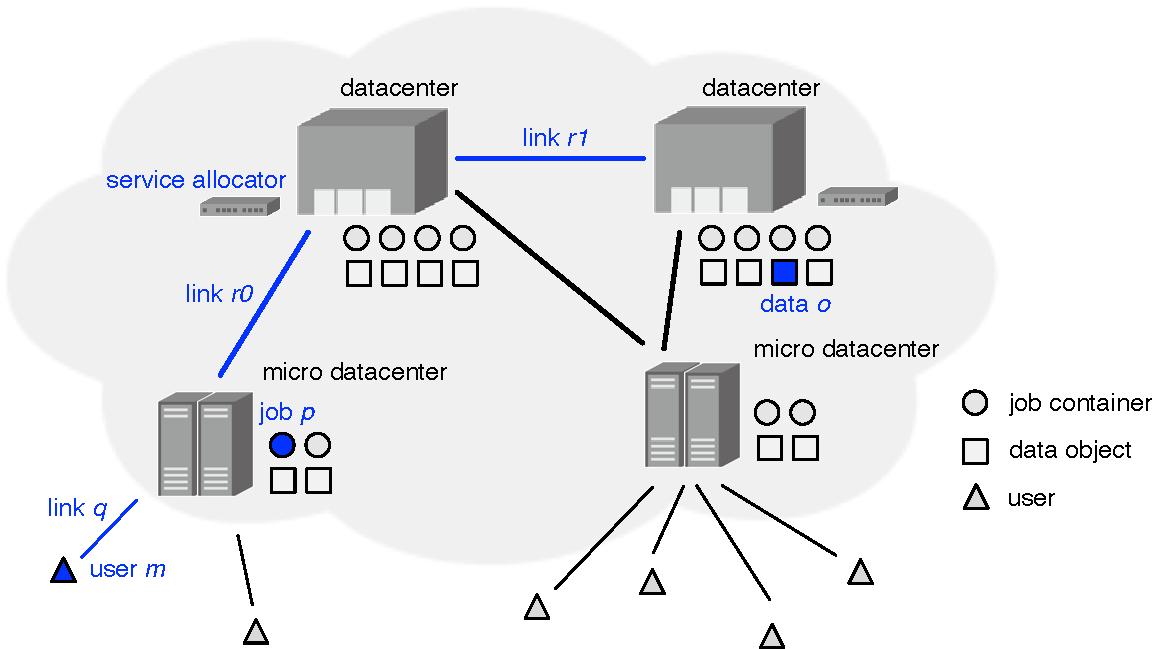
\includegraphics[width=1.0\columnwidth]{system.pdf}
    \vspace{-2.0ex}
    \caption{Simple system model}
    \Description{A simple system model with 2 datacenters and 2 micro datacenters.}
    \label{fig:system}
  \end{center}
\end{figure}

Our resource management model is explained using a simple system
configuration with 2 datacenters (DCs) and 2 micro-datacenters (MDCs)
shown in Figure~\ref{fig:system}.
When a user requests a service to a nearby service allocation server,
the service server instantiates the requested service into a series of
microservice jobs.
The server finds the required resources for each job,
identifies the locations of the user and the required data object,
asks resource agents for available resources and their current costs,
and assigns the job to the node that minimizes the total cost for the
job.
The area for cost inquiry could be within proximity along the path
between the user and the data object.

The load of a resource can be measured in a number of ways.  Most
resources have some form of load report functions built-in.
When the load of a resource fluctuates too rapidly,
a smoothing filter (e.g., exponentially weighted moving average)
can be used to stabilize the behavior.
A load value does not need to be precise, and a rough approximation is
enough for loose resource management.
Still, if each allocation is not small enough both in size and in
duration, the loads may not converge as expected.
Therefore, microservice is the enabler for this approach.

\subsection{Job Assignment}

In this paper, we use a simple micro-job model that defines the
required resources for a micro-job as $J(p, q, r, s)$ where 
$p$ is the number of micro containers for computation, 
$q$ is frontend communication with the user, 
$r$ is backend communication with data objects (e.g., database), and
$s$ is the number of time slots.
%%The unit is one micro-container for $p$, 1Mbps for $q$ and $r$, and 1
%%second for $s$.
The communication costs $q$ and $r$ are also a function of distance so
that an interactive job with $q \gg r$ will be placed close to the
user and a data-intensive jobs with $q \ll r$ will be placed close to
the data.
For simplicity, we do not distinguish directions of
communications for $q$ and $r$, and assume only one user and one data
object per job in this paper.

A job is specified by a service provider, optionally associated with
weights, e.g., a service provider may raise the weight for the
frontend communication to place the job close to the user.
In this manner, cloud service providers can specify which
type of resources have a priority for a specific service without
overclaiming required resources.

To instantiate a micro-job requested from a user, the service
server finds the best node to allocate the required resource
for $J$: $p$, $q$ and $r$ for duration $s$.

The pseudo cost $E$ to host job $j$ for a unit time at node $i$ for
user $m$ and data object $o$ is:
\begin{equation*}
	E(j, i)     = H(j,i) + G(j,i,m,o)
\end{equation*}
here, $H(j, i)$ is the computing cost to run $j$ at $i$, and
$G(j, i, m, o)$ is the communication cost to run $j$ at $i$
between $m$ and $o$.
\begin{eqnarray*}
&&  H(j,i)      = p \cdot f(\rho_{i}) \\
&&  G(j,i,m,o)  = q \cdot \smashoperator{\sum_{l \in path(m,i)}} f(\rho_{l}) + r \cdot \smashoperator{\sum_{l \in path(i,o)}} f(\rho_{l})
\end{eqnarray*}
$f(\rho)$ is the cost function of a resource load, and $path(m,i)$ is a set
of links from $m$ to $i$ (e.g., the shortest path weighted by cost).

To assign Job $j$, the server simply finds the node that minimizes the
cost:
\begin{equation*}
	argmin_{i} \: E(j, i)
\end{equation*}

\subsection{Pseudo Cost Functions}

%% idea: mechanics model instead of optimization

Our model employs a parametric representation of pseudo cost, as a
function of load, and uses it for load control and also as
backpressure against congestion.
Micro-jobs are naturally gravitated to the most cost-efficient
location.

%% model: cost function: congestion pricing combined with idle-resource pooling
The proposed model is based on congestion pricing in which the cost of
a resource dynamically changes according to the load of the resource.
It works as a barrier function for optimization; the capacity
constraint is enforced by a penalizing cost when approaching the full
capacity.

Another key idea is {\em idle-resource pooling} that tries to put resources
into an idle state when possible for energy saving.
We proposed a convex cost function that enables idle-resource pooling
as part of the congestion pricing mechanism.

A pseudo cost function in our model maps the load of a resource
$\rho \in [0, 1]$ to the corresponding cost.
The capacity limit is enforced by the cost function that rapidly grows
as the load approaches $1.0$, which is known as a barrier function in
optimization theory. 

We use two types of pseudo cost functions: one is the monotonic cost
function and the other is the convex cost function.
The monotonic cost function is a simple barrier function that
monotonically grows with load, up to infinite as $\rho \to 1$.
The convex cost function is also a barrier function but also for
idle-resource pooling.
In this paper, the monotonic form is used for network links as
energy-saving-by-idling is not common for network links.

The standard forms that have the minimum cost of $1.0$ are
shown in Figure~\ref{fig:std_costfunc}. We will show how to manipulate
the cost functions in Sec.~\ref{sec:variation}.

\begin{figure}[tb]
  \begin{center}
    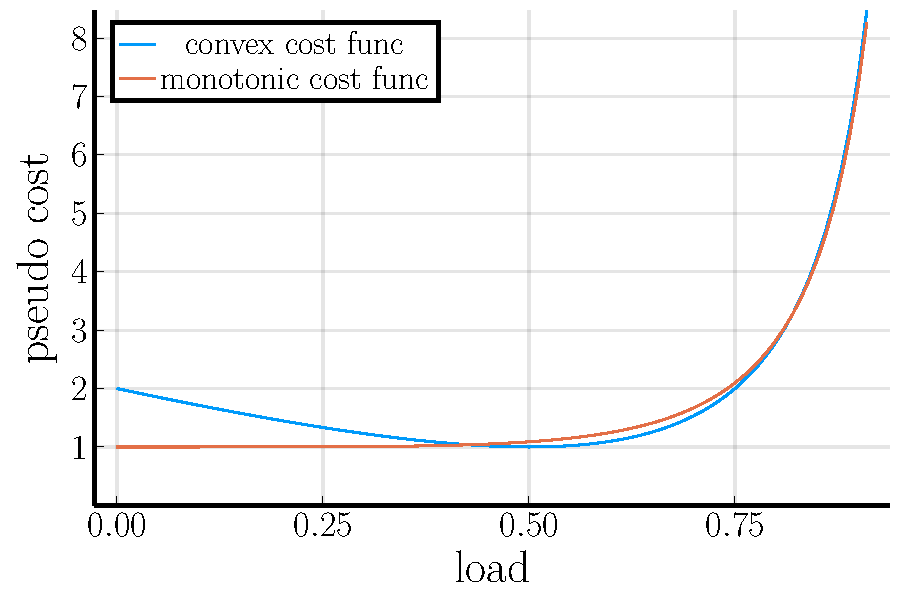
\includegraphics[width=0.9\columnwidth]{pseudo_costs.pdf}
    \vspace{-2.0ex}
    \caption{Standard cost functions}
    \Description{The standard convex cost function and standard
      monotonic cost function.}
    \label{fig:std_costfunc}
  \end{center}
\end{figure}

The standard convex cost function is defined as:
\begin{equation*}
	f(\rho) = \frac{(2\rho - 1)^{2}}{1 - \rho} + 1
\end{equation*}
This function has the properties:
$min\: f(\rho) = f(.5) = 1$, and $f(0) = f(.75) = 2$.
The cost grows rapidly when $\rho > .75$.
The system automatically tries to keep $\rho \le .75$,
aiming at $\rho = .5$.

The standard monotonic cost function is defined as:
\begin{equation*}
	f(\rho) = \frac{\rho^{4.5}}{1 - \rho} + 1
\end{equation*}
to roughly match the standard convex cost function in $[.5, .75]$,
the {\em working load range} explained in the next subsection.

Note that the standard forms are defined just for convenience, and
other functions with a similar shape in $[0,1]$ also work for our
purposes.

\subsection{Idle-Resource Pooling in Action}

The behavior of idle-resource pooling by the convex cost function is
illustrated by the following examples in Figure~\ref{fig:4node} and
Figure~\ref{fig:4node-ratio}.

\begin{figure}[tb]
  \begin{center}
    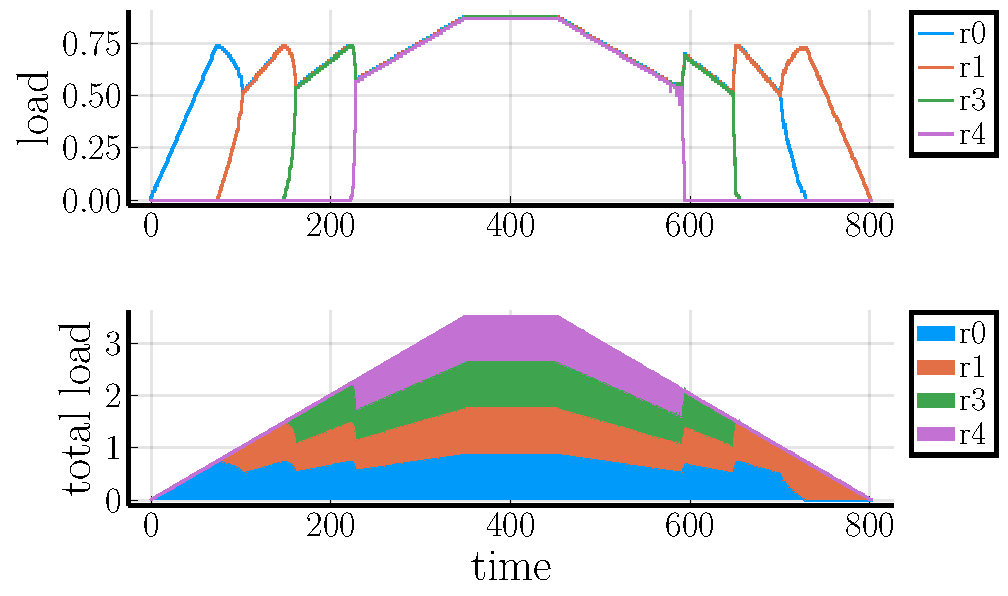
\includegraphics[width=1.0\columnwidth]{equivalent_nodes.pdf}
    \vspace{-2.0ex}
    \caption{Load distribution among 4 equivalent cost nodes:
    the load of each resource (top) and the total load (bottom)}
    \Description{Simulation results with 4 nodes with the same cost function.}
    \label{fig:4node}
  \end{center}
  \hspace{0.8\columnsep}
\end{figure}

First, assume a pool of 4 equivalent resources with the standard convex
cost function.
Also, assume that micro-jobs are continuously assigned to the
system; each micro-job is much smaller than the capacity of a
resource.

The initial system load $\sum \rho$ is $0$, and gradually increased up
to $3.5$ until time 350. After time 400, the system load is gradually
decreased back to $0$ until time 750.
Here, load $1.0$ is the capacity of a single resource. 
Initially, all resources in the pool are idle, and their costs are
all $f(0)= 2$.
For the first job, one resource $r_{0}$ is randomly selected for allocation, and its
cost becomes lower: $f(0+) < 2$. As a result, subsequent jobs are
assigned to $r_{0}$, with lowering cost towards $\rho = .5$ and then
rising again until $\rho = .75$ where $f(.75) = 2 = f(0)$.
At this point, another resource $r_{1}$ is selected for allocation.
$r_{1}$ is preferred over $r_{0}$ as its cost becomes lower with new
allocations so that both loads move towards $\rho_{0} = \rho_{1} = .5$,
where both are balanced.
Both loads rise again until $\rho_{r0} = \rho_{r1} = .75$,
where the third resource $r_{2}$ kicks in.
It repeats for $r_{3}$, but no more idle resource is available
when $\sum \rho$ reaches $3.0$ so that the loads grow beyond $.75$
up to $\sum \rho = 3.5$ with $\rho = .875$ for each.

When the system load decreases, the process is reversed.
After reaching $\rho = .5$ for all,
one resource with the lowest load $\rho < .5$ becomes more expensive
than the others.
This one is less preferred for subsequent assignments, and quickly
loses the load until it becomes idle again, while the other 3 keep
$\rho$ in $[.5, .75]$. It repeats for the remaining ones.

It is easy to see how the number of active resources changes when
there are more resources.
When the number of active resources is increasing, the load of each
active resource stay at around $\rho = .75$.
On the other hand, when the number of active resources is decreasing,
the load of each active resource stay at around $\rho = .5$.
In short, when all resources are equal, the system tries to maintain
the load of active resources in the {\em working load range}
$[.5, .75]$, while keeping idle resources as much as possible.

\begin{figure}
  \begin{center}
    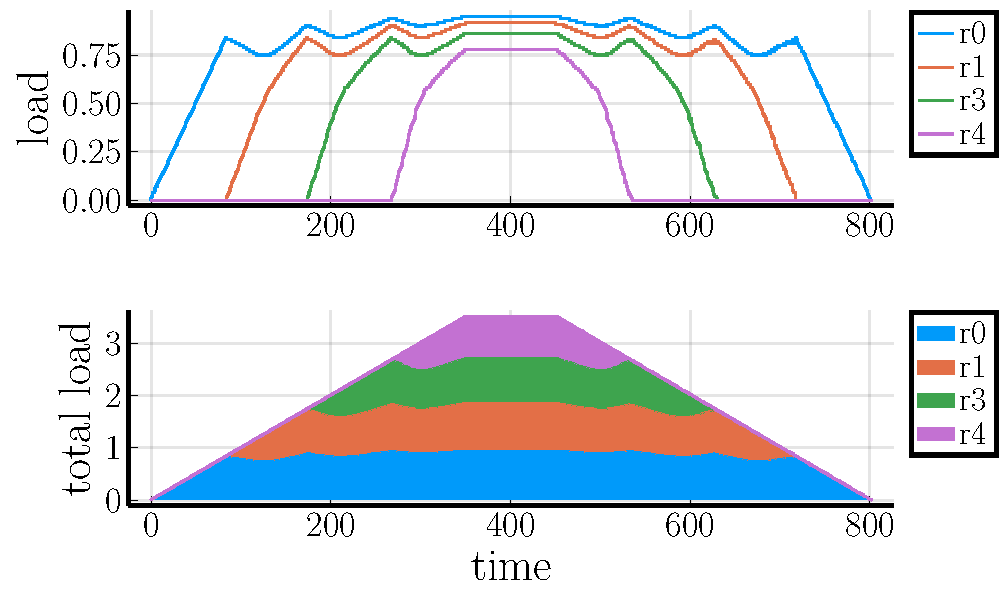
\includegraphics[width=1.0\columnwidth]{proportional_nodes.pdf}
    \vspace{-2.0ex}
    \caption{Load distribution: 4 proportional cost nodes}
    \Description{Simulation results with 4 nodes with proportional cost functions.}
    \label{fig:4node-ratio}
  \end{center}
\end{figure}

When resources are not equal, the behavior becomes more complex, but
the underlying mechanisms are the same.
Let's take a look at a case of 4 resources in Figure~\ref{fig:4node-ratio}
with the cost ratio $1:2:4:8$,
that is $8 f_{r0} = 4 f_{r1} = 2 f_{r2} = f_{r3}$.
Here, we focus on the interaction between $r_{0}$ and $r_{1}$ since
the other interactions are similar.
To activate $r_{1}$, the load of $r_{0}$ goes up to $.84$ to satisfy:
$f_{r1}(0) = 4 = f_{r0}(.84)$.
When $r_{1}$ is moving towards idle after time 550, the load
of $r_{0}$ is $.75$ to satisfy: $f_{r1}(.5) = 2 = f_{r0}(.75)$

For unequal resources in general, the required load to trigger a new
allocation is higher than $\rho = .75$ for the already
active ones to match the cost $f(0)$ for the new one, but the load
will not go much further as the slope of the cost function is steep.
Similarly, when the most expensive one among active resources becomes
idle, the load of the remaining ones stay at the matching cost 
$f(.5)$ for the deactivating one.

%%Note that our goal is not to achieve the theoretical optimum but to
%%enable loose automatic distributed load balancing.

\subsection{Manipulating the Cost Function}
\label{sec:variation}

The utilization of a resource can be manipulated by modifying the cost
function of the resource as shown in Figure~\ref{fig:costfunc3}.

One can {\bf lower or raise the load level} of a resource by shifting
the load in the cost function and adjusting the target load,
$f'(\rho) = f(\rho + \Delta)$.

To {\bf change the activation order} in the idlle-resource pooling,
one can raise or lower the cost,
e.g., by making the cost  $n$ times more expensive, $f'(\rho) = n f(\rho)$.
For minor adjustment, one can use an additive form,
$f'(\rho) = f(\rho) + \Delta$.

To make {\bf idle-resource pooling more aggressive},
one can raise the cost at $\rho = 0$:
e.g., to raise the cost at $\rho = 0$ by a factor of $(n+1)/2$,
$f'(\rho) = n (2\rho - 1)^{2}/(1 - \rho^{n}) + 1$.

A {\bf premium service} can be realized by shifting the load
in the same way as lowering the load level
but for specific users or jobs (not for a specific resource) so as to
have premium jobs always being assigned to less loaded resources.
Similarly, an {\bf economy service} that allows to be assigned to more
loaded resources can be made by a negative shift.
It could be appealing to enable multiple classes using a single
resource pool with a single shift parameter.

\begin{figure}[tb]
  \begin{center}
    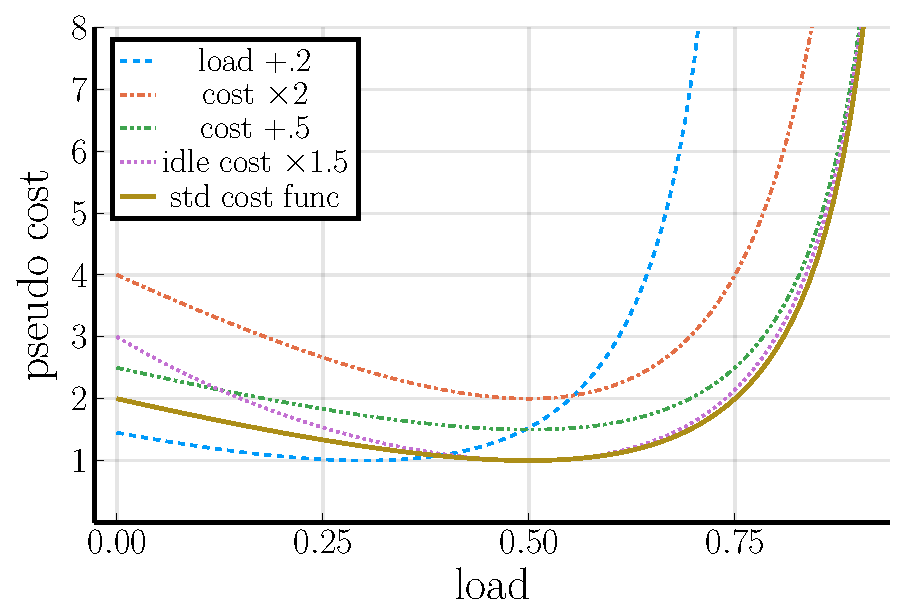
\includegraphics[width=0.9\columnwidth]{pseudo_costs_2.pdf}
    \vspace{-2.0ex}
    \caption{Manipulating convex cost functions}
    \Description{Variations of manipulated cost functions are shown.}
    \label{fig:costfunc3}
  \end{center}
\end{figure}

Other than manipulating the cost function,
cloud service providers can adjust the required resources and their
weights for a job.  Also, it is effective to place data objects close to the
users, and both service providers and their users should have some
control over where to store the data.
Thus, the system allows stakeholders to loosely control the
resource utilization.
